\newpage 

\ifnum \Version=1  
\question[7] Consider the system $$\vec x \, ' = A\vec x, \quad A = \begin{pmatrix} 0&3\\5&2 \end{pmatrix}, \quad \vec x = \begin{pmatrix} x(t)\\y(t)\end{pmatrix} $$.
\begin{parts}
    \part Determine the eigenvalues of $A$. Please show your work. \vspace{5cm}
    \part Determine the eigenvectors of $A$. Please show your work. \vspace{7cm}
    \part Sketch the phase portrait of the system on the axes below. Please indicate the direction of motion on your solution curves and draw the eigenspaces corresponding to real eigenvalues (if any). Please also label your axes. 
    \begin{center}
    \begin{tikzpicture}[scale=0.85]
    \draw[very thick, ->] (-3, 0) -- (3.25, 0);
    \draw[very thick, ->] (0, -3) -- (0, 3.25);
    \end{tikzpicture}
    \end{center}
\end{parts}
\fi

\ifnum \Version=2
\question[7] Consider the system $$\vec x \, ' = A\vec x, \quad A = \begin{pmatrix} 4&3\\3&-4 \end{pmatrix}, \quad \vec x = \begin{pmatrix} x(t)\\y(t)\end{pmatrix} $$.
\begin{parts}
    \part Determine the eigenvalues of $A$. Please show your work. \vspace{5cm}
    \part Determine the eigenvectors of $A$. Please show your work. \vspace{7cm}
    \part Sketch the phase portrait of the system on the axes below. Please indicate the direction of motion on your solution curves and draw the eigenspaces corresponding to real eigenvalues (if any). Please also label your axes. 
    \begin{center}
    \begin{tikzpicture}[scale=0.85]
    \draw[very thick, ->] (-3, 0) -- (3.25, 0);
    \draw[very thick, ->] (0, -3) -- (0, 3.25);
    \end{tikzpicture}
    \end{center}
\end{parts}
\fi

\ifnum \Version=3
\question[7] Consider the system $$\vec x \, ' = A\vec x, \quad A = \begin{pmatrix} 5&4\\-3&-3 \end{pmatrix}, \quad \vec x = \begin{pmatrix} x(t)\\y(t)\end{pmatrix} $$.
\begin{parts}
    \part Determine the eigenvalues of $A$. Please show your work. \vspace{5cm}
    \part Determine the eigenvectors of $A$. Please show your work. \vspace{7cm}
    \part Sketch the phase portrait of the system on the axes below. Please indicate the direction of motion on your solution curves and draw the eigenspaces corresponding to real eigenvalues (if any). Please also label your axes. 
    \begin{center}
    \begin{tikzpicture}[scale=0.85]
    \draw[very thick, ->] (-3, 0) -- (3.25, 0);
    \draw[very thick, ->] (0, -3) -- (0, 3.25);
    \end{tikzpicture}
    \end{center}
\end{parts}
\fi

\ifnum \Version=4
\question[7] Consider the system $$\vec x \, ' = A\vec x, \quad A = \begin{pmatrix} 3&4\\-3&-5 \end{pmatrix}, \quad \vec x = \begin{pmatrix} x(t)\\y(t)\end{pmatrix} $$.
\begin{parts}
    \part Determine the eigenvalues of $A$. Please show your work. \vspace{5cm}
    \part Determine the eigenvectors of $A$. Please show your work. \vspace{7cm}
    \part Sketch the phase portrait of the system on the axes below. Please indicate the direction of motion on your solution curves and draw the eigenspaces corresponding to real eigenvalues (if any). Please also label your axes. 
    \begin{center}
    \begin{tikzpicture}[scale=0.85]
    \draw[very thick, ->] (-3, 0) -- (3.25, 0);
    \draw[very thick, ->] (0, -3) -- (0, 3.25);
    \end{tikzpicture}
    \end{center}
\end{parts}
\fi

\ifnum \Version=5
\question[7] Consider the system $$\vec x \, ' = A\vec x, \quad A = \begin{pmatrix} 4&4\\-3&-4 \end{pmatrix}, \quad \vec x = \begin{pmatrix} x(t)\\y(t)\end{pmatrix} $$.
\begin{parts}
    \part Determine the eigenvalues of $A$. Please show your work. \vspace{5cm}
    \part Determine the eigenvectors of $A$. Please show your work. \vspace{7cm}
    \part Sketch the phase portrait of the system on the axes below. Please indicate the direction of motion on your solution curves and draw the eigenspaces corresponding to real eigenvalues (if any). Please also label your axes. 
    \begin{center}
    \begin{tikzpicture}[scale=0.85]
    \draw[very thick, ->] (-3, 0) -- (3.25, 0);
    \draw[very thick, ->] (0, -3) -- (0, 3.25);
    \end{tikzpicture}
    \end{center}
\end{parts}
\fi



\ifnum \Version=6
    \question[6] Consider the IVP $$\vec x \, ' = A\vec x, \quad A = \begin{pmatrix} -1&3\\3&-1 \end{pmatrix}, \quad \vec x = \begin{pmatrix} x(t)\\y(t)\end{pmatrix}, \quad \vec x(0) = \begin{pmatrix} 2\\2 \end{pmatrix}$$ The eigenvalues of $A$ are $\lambda_1 = -4$ and $\lambda_2 = 2$. 
    \begin{parts}
        \part Determine the eigenvectors of $A$. Please show your work. 
        
        \ifnum \Solutions=1 {\color{DarkBlue} 
        \textbf{Solutions:}
        For $\lambda_1$:
        \begin{align}
            A - \lambda_1 I = \begin{pmatrix} 3&3\\3&3\end{pmatrix} \ \Rightarrow \ v_1 = \begin{pmatrix} -1\\1 \end{pmatrix}
        \end{align}
        For $\lambda_2$:
        \begin{align}
            A - \lambda_2 I = \begin{pmatrix} -3&3\\3&-3\end{pmatrix} \ \Rightarrow \ v_2 = \begin{pmatrix} 1\\1 \end{pmatrix}
        \end{align}    
        } 
        \else 
            \vspace{6cm}   
        \fi        
        \part Use the given eigenvalues and the eigenvectors that you calculated in part (a) to solve the IVP.  
        
        \ifnum \Solutions=1 {\color{DarkBlue} 
        \textbf{Solutions:} the general solution to the DE is:
        $$\vec x = c_1 e^{-4t}\begin{pmatrix} -1\\1\end{pmatrix} + c_2e^{2t} \begin{pmatrix} 1\\1\end{pmatrix}$$
        Use initial condition:
        \begin{align}
            \begin{pmatrix} 2\\2\end{pmatrix} &= c_1\begin{pmatrix}-1\\1 \end{pmatrix}+ c_2 \begin{pmatrix} 1\\1\end{pmatrix} \ \Rightarrow \ c_1 = 0, c_2 = 2 \ \Rightarrow \ 
            \vec x (t) = 2e^{2t} \begin{pmatrix} 1\\1\end{pmatrix}
        \end{align}
        } 
        \else 
        \vspace{7cm}
    \fi
    \part Sketch the phase portrait of the system on the axes below. Please indicate the direction of motion on your solution curves and draw the eigenspaces corresponding to real eigenvalues (if any). Please also label your axes. 
    
    \ifnum \Solutions=1 {\color{DarkBlue} 
    \textbf{Solutions:}
        \begin{center}
        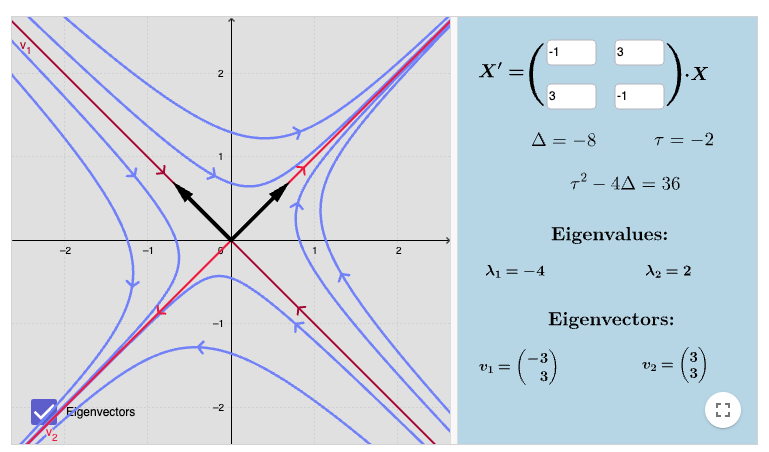
\includegraphics[width=5in]{Images/ImgPhasePlane1331.png}
        \end{center}         
    } 
    \else 
        \begin{center}
        \begin{tikzpicture}[scale=0.85]
        \draw[very thick, ->] (-3, 0) -- (3.25, 0);
        \draw[very thick, ->] (0, -3) -- (0, 3.25);
        \end{tikzpicture}
        \end{center}    
    \fi    

\end{parts}
\fi





\ifnum \Version=7
    \question[6] Consider the IVP $$\vec x \, ' = A\vec x, \quad A = \begin{pmatrix} 0&3\\3&8 \end{pmatrix}, \quad \vec x = \begin{pmatrix} x(t)\\y(t)\end{pmatrix}, \quad \vec x(0) = \begin{pmatrix} -3\\1 \end{pmatrix}$$ The eigenvalues of $A$ are $\lambda_1 = -1$ and $\lambda_2 = 9$. 
    \begin{parts}
        \part Determine the eigenvectors of $A$. Please show your work. 
        
        \ifnum \Solutions=1 {\color{DarkBlue} 
        \textbf{Solutions:}
        For $\lambda_1$:
        \begin{align}
            A - \lambda_1 I = \begin{pmatrix} 1&3\\3&9\end{pmatrix} \ \Rightarrow \ v_1 = \begin{pmatrix} -3\\1 \end{pmatrix}
        \end{align}
        For $\lambda_2$:
        \begin{align}
            A - \lambda_2 I = \begin{pmatrix} -9&3\\3&-1\end{pmatrix} \ \Rightarrow \ v_2 = \begin{pmatrix} 1\\3 \end{pmatrix}
        \end{align}    
        } 
        \else 
            \vspace{6cm}   
        \fi        
        \part Use the given eigenvalues and the eigenvectors that you calculated in part (a) to solve the IVP.  
        
        \ifnum \Solutions=1 {\color{DarkBlue} 
        \textbf{Solutions:} the general solution to the DE is:
        $$\vec x = c_1 e^{-t}\begin{pmatrix} -3\\1\end{pmatrix} + c_2e^{9t} \begin{pmatrix} 1\\3\end{pmatrix}$$
        Use initial condition:
        \begin{align}
            \begin{pmatrix} -3\\1\end{pmatrix} &= c_1\begin{pmatrix}-3\\1 \end{pmatrix}+ c_2 \begin{pmatrix} 1\\3\end{pmatrix} \ \Rightarrow \ c_1 = 1, c_2 = 0 \ \Rightarrow \ 
            \vec x (t) = e^{-t} \begin{pmatrix} -3\\1\end{pmatrix}
        \end{align}
        } 
        \else 
        \vspace{7cm}
    \fi
    \part Sketch the phase portrait of the system on the axes below. Please indicate the direction of motion on your solution curves and draw the eigenspaces corresponding to real eigenvalues (if any). Please also label your axes. 
    
    \ifnum \Solutions=1 {\color{DarkBlue} 
    \textbf{Solutions:}
        \begin{center}
        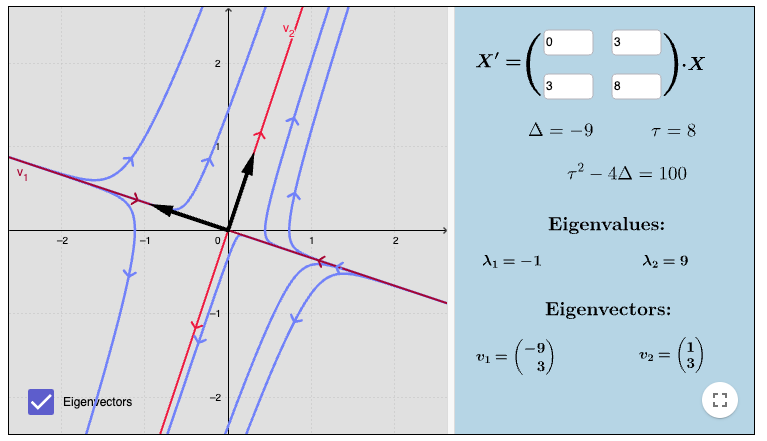
\includegraphics[width=5in]{Images/ImgPhasePlane0338.png}
        \end{center}         
    } 
    \else 
        \begin{center}
        \begin{tikzpicture}[scale=0.85]
        \draw[very thick, ->] (-3, 0) -- (3.25, 0);
        \draw[very thick, ->] (0, -3) -- (0, 3.25);
        \end{tikzpicture}
        \end{center}    
    \fi    

\end{parts}
\fi








\ifnum \Version=8
    \question[6] Consider the IVP $$\vec x \, ' = A\vec x, \quad A = \begin{pmatrix} -1&3\\3&7 \end{pmatrix}, \quad \vec x = \begin{pmatrix} x(t)\\y(t)\end{pmatrix}, \quad \vec x(0) = \begin{pmatrix} 1\\3 \end{pmatrix}$$ The eigenvalues of $A$ are $\lambda_1 = -2$ and $\lambda_2 = 8$. 
    \begin{parts}
        \part Determine the eigenvectors of $A$. Please show your work. 
        
        \ifnum \Solutions=1 {\color{DarkBlue} 
        \textbf{Solutions:}
        For $\lambda_1$:
        \begin{align}
            A - \lambda_1 I = \begin{pmatrix} 1&3\\3&9\end{pmatrix} \ \Rightarrow \ v_1 = \begin{pmatrix} -3\\1 \end{pmatrix}
        \end{align}
        For $\lambda_2$:
        \begin{align}
            A - \lambda_2 I = \begin{pmatrix} -9&3\\3&-1\end{pmatrix} \ \Rightarrow \ v_2 = \begin{pmatrix} 1\\3 \end{pmatrix}
        \end{align}    
        } 
        \else 
            \vspace{6cm}   
        \fi        
        \part Use the given eigenvalues and the eigenvectors that you calculated in part (a) to solve the IVP.  
        
        \ifnum \Solutions=1 {\color{DarkBlue} 
        \textbf{Solutions:} the general solution to the DE is:
        $$\vec x = c_1 e^{-4t}\begin{pmatrix} -1\\1\end{pmatrix} + c_2e^{2t} \begin{pmatrix} 1\\1\end{pmatrix}$$
        Use initial condition:
        \begin{align}
            \begin{pmatrix} 1\\3\end{pmatrix} &= c_1\begin{pmatrix}-3\\1 \end{pmatrix}+ c_2 \begin{pmatrix} 1\\3\end{pmatrix} \ \Rightarrow \ c_1 = 0, c_2 = 1 \ \Rightarrow \ 
            \vec x (t) = e^{8t} \begin{pmatrix} 1\\3\end{pmatrix}
        \end{align}
        } 
        \else 
        \vspace{7cm}
    \fi
    \part Sketch the phase portrait of the system on the axes below. Please indicate the direction of motion on your solution curves and draw the eigenspaces corresponding to real eigenvalues (if any). Please also label your axes. 
    
    \ifnum \Solutions=1 {\color{DarkBlue} 
    \textbf{Solutions:}
        \begin{center}
        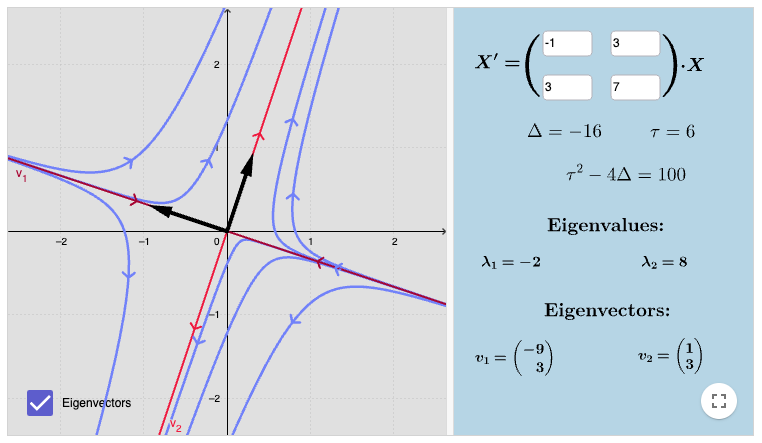
\includegraphics[width=5in]{Images/ImgPhasePlane1337.png}
        \end{center}         
    } 
    \else 
        \begin{center}
        \begin{tikzpicture}[scale=0.85]
        \draw[very thick, ->] (-3, 0) -- (3.25, 0);
        \draw[very thick, ->] (0, -3) -- (0, 3.25);
        \end{tikzpicture}
        \end{center}    
    \fi    

\end{parts}
\fi








\ifnum \Version=9
    \question[6] Consider the IVP $$\vec x \, ' = A\vec x, \quad A = \begin{pmatrix} -2&3\\3&-2 \end{pmatrix}, \quad \vec x = \begin{pmatrix} x(t)\\y(t)\end{pmatrix}, \quad \vec x(0) = \begin{pmatrix} 2\\2 \end{pmatrix}$$ The eigenvalues of $A$ are $\lambda_1 = -5$ and $\lambda_2 = 1$. 
    \begin{parts}
        \part Determine the eigenvectors of $A$. Please show your work. 
        
        \ifnum \Solutions=1 {\color{DarkBlue} 
        \textbf{Solutions:}
        For $\lambda_1$:
        \begin{align}
            A - \lambda_1 I = \begin{pmatrix} 3&3\\3&3\end{pmatrix} \ \Rightarrow \ v_1 = \begin{pmatrix} -1\\1 \end{pmatrix}
        \end{align}
        For $\lambda_2$:
        \begin{align}
            A - \lambda_2 I = \begin{pmatrix} -3&3\\3&-3\end{pmatrix} \ \Rightarrow \ v_2 = \begin{pmatrix} 1\\1 \end{pmatrix}
        \end{align}    
        } 
        \else 
            \vspace{6cm}   
        \fi        
        \part Use the given eigenvalues and the eigenvectors that you calculated in part (a) to solve the IVP.  
        
        \ifnum \Solutions=1 {\color{DarkBlue} 
        \textbf{Solutions:} the general solution to the DE is:
        $$\vec x = c_1 e^{-5t}\begin{pmatrix} -1\\1\end{pmatrix} + c_2e^{t} \begin{pmatrix} 1\\1\end{pmatrix}$$
        Use initial condition:
        \begin{align}
            \begin{pmatrix} 2\\2\end{pmatrix} &= c_1\begin{pmatrix}-1\\1 \end{pmatrix}+ c_2 \begin{pmatrix} 1\\1\end{pmatrix} \ \Rightarrow \ c_1 = 0, c_2 = 2 \ \Rightarrow \ 
            \vec x (t) = 2e^{t} \begin{pmatrix} 1\\1\end{pmatrix}
        \end{align}
        } 
        \else 
        \vspace{7cm}
    \fi
    \part Sketch the phase portrait of the system on the axes below. Please indicate the direction of motion on your solution curves and draw the eigenspaces corresponding to real eigenvalues (if any). Please also label your axes. 
    
    \ifnum \Solutions=1 {\color{DarkBlue} 
    \textbf{Solutions:}
        \begin{center}
        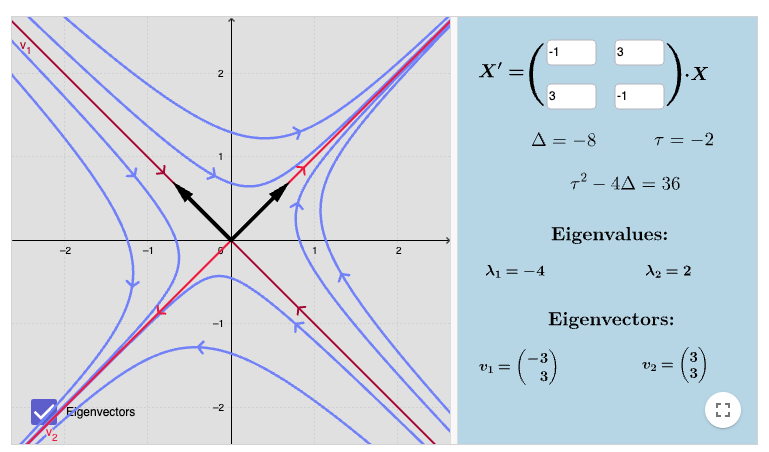
\includegraphics[width=5in]{Images/ImgPhasePlane1331.png}
        \end{center}         
    } 
    \else 
        \begin{center}
        \begin{tikzpicture}[scale=0.85]
        \draw[very thick, ->] (-3, 0) -- (3.25, 0);
        \draw[very thick, ->] (0, -3) -- (0, 3.25);
        \end{tikzpicture}
        \end{center}    
    \fi    

\end{parts}
\fi